\documentclass[11pt]{beamer}
\usepackage{helvet} %font
\beamertemplatenavigationsymbolsempty
\usetheme{JuanLesPins}
\usefonttheme{structurebold}

\usepackage[french]{babel}
\usepackage[utf8]{inputenc}
\usepackage[T1]{fontenc}
\usepackage{amssymb,amsmath}
\usepackage{tikz}
\usepackage{geometry}
\usepackage{xcolor,colortbl}
\usetikzlibrary{arrows,positioning}
\usepackage{listings}

\AtBeginSubsection[]
{
   \begin{frame}
	\small \tableofcontents[currentsection]
   \end{frame}
}

\newenvironment{slide}[1]{%
\begin{frame}[environment=slide]
\frametitle{#1}
}{%
\end{frame}
}
\setbeamercolor{structure}{fg=red}
\setbeamercolor{frametitle}{bg=black,fg=white}
\definecolor{gris}{gray}{0.6}
\definecolor{grisclair}{gray}{0.9}

\newtheorem{exercice}{Exercice}

\title{Machine Learning VIII : Minimisation du risque}
\author{Nicolas Bourgeois}
\date{}

\newcommand{\Python}[1]{
	{\small	\lstinputlisting[language=Python]{./#1.py}}
}
\newenvironment{pyenvsmall}
	{ \ttfamily \tiny }
	{\par  }

\newcommand{\Pythonsmall}[1]{
	{\scriptsize \lstinputlisting[language=Python]{./#1.py}}
}
\newcommand{\elimine}[1]{{\textcolor{lightgray}{#1}}}

\newcommand\Wider[2][3em]{%
\makebox[\linewidth][c]{%
  \begin{minipage}{\dimexpr\textwidth+#1\relax}
  \raggedright#2
  \end{minipage}%
  }%
}

\begin{document}

\begin{frame}
\maketitle
\end{frame}

\begin{frame}
\tableofcontents
\end{frame}


\section{Outils de base}

\subsection{Fonction de Perte} 

\begin{frame}{Fonction de Perte}
Soit $LF:E \rightarrow \mathbb{R}_+$ une fonction de perte, telle que
$$LF(Y,Y) = 0$$\\
Et $\Phi$ une fonction d'agrégation

Objectif :
$$ \min_f \Phi \left( LF(f(X_i),Y_i) \right)$$

\end{frame}

\begin{frame}{Exercice}
\begin{exercice}
Suggérez des fonctions de perte pour la régression
\end{exercice}

\vspace{0.3cm}

\begin{exercice}
Suggérez des fonctions de perte pour la classification
\end{exercice}
\end{frame}

\begin{frame}{Solution}
1)\\
$LF(X,Y) = (X-Y)^q$\\
$LF(X,Y) = \frac{|X-Y|}{|X+Y|}$\\
\vspace{0.3cm}
2)\\

$LF(X,Y) = \mathbf{1}_{X\neq Y}$\\
$LF(X,Y) = 1$ si $X>Y$, $\epsilon$ si $X<Y$, $0$ sinon.  

\end{frame}

\subsection{Risque empirique}

\begin{frame}{Risque empirique}
Soit $LF:E \rightarrow \mathbb{R}_+$ une fonction de perte, telle que
$$LF(Y,Y) = 0$$\\
Et on fait la moyenne \textit{sur l'échantillon observé}:

Objectif :
$$ \frac{1}{N}\sum_{i \in I} \left( LF(f(X_i),Y_i) \right)$$

\end{frame}


\begin{frame}{Exercice}
\begin{exercice}
En reprenant les données iris, programmez (sans utiliser scipy ou scikit-learn) une régression linéaire entre la longueur et l'épaisseur des pétales, en choisissant respectivement :
\begin{itemize}
	\item $LF(X,Y) = (X-Y)^2$
	\item $LF(X,Y) = |X-Y|$
\end{itemize}
Affichez les deux droites sur le même graphe.
\end{exercice}

\end{frame}

\begin{frame}{Résultat attendu}
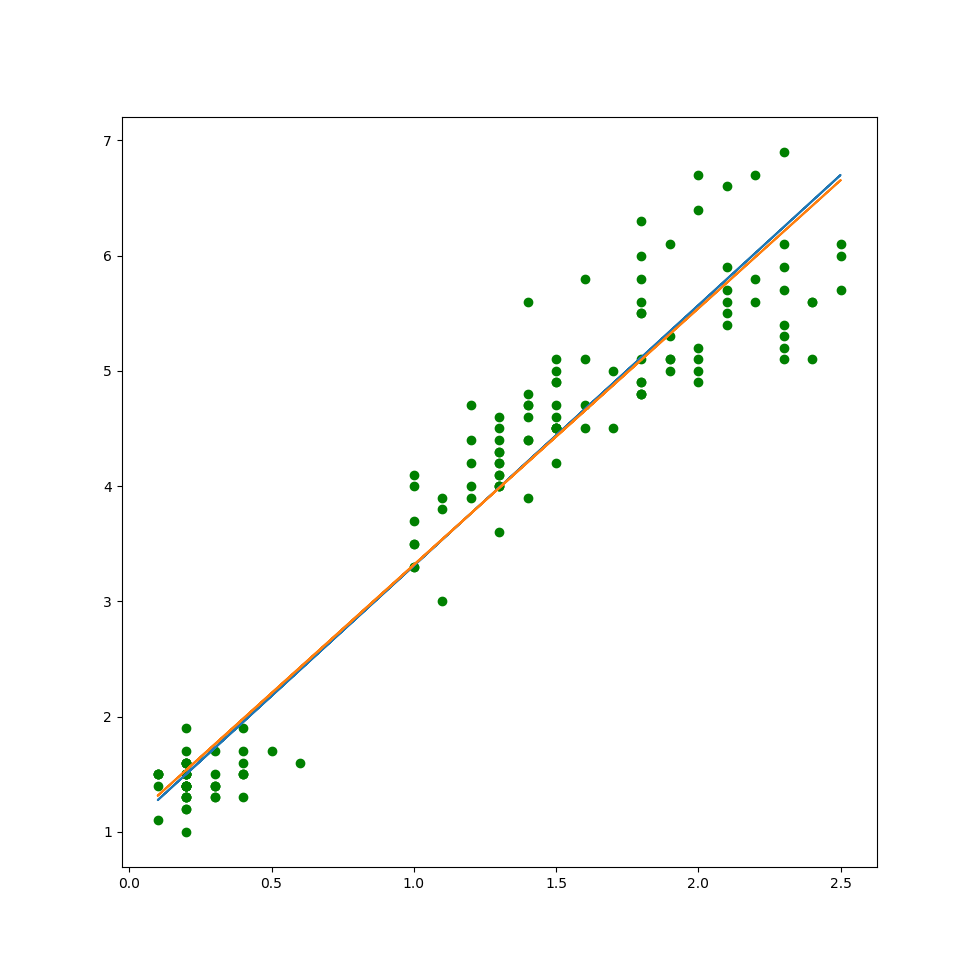
\includegraphics[scale=0.3]{ext1}
\end{frame}

\begin{frame}{Solution}
\Pythonsmall{ext1}
\end{frame}

\begin{frame}{Exercice}
\begin{exercice}
Construisez un exemple pour lequel le choix de la fonction de perte a un gros impact sur la régression.
\end{exercice}
\end{frame}

\begin{frame}{Solution}
\Pythonsmall{ext2}
\end{frame}

\begin{frame}{Solution}
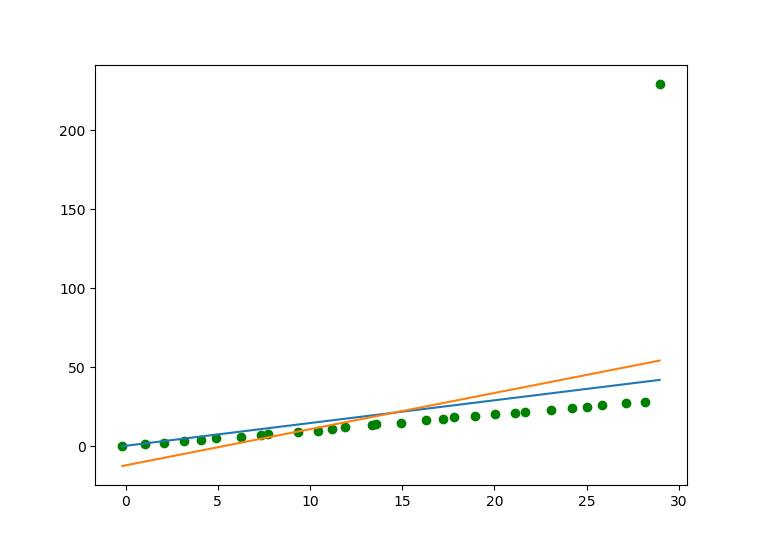
\includegraphics[scale=0.4]{ext2}
\end{frame}


\subsection{Matrice de confusion}

\begin{frame}{Principe}
Dans le cas d'une classification supervisée, on considère:

$$c_{jk} = |i,g(X_i)=j \& Y_i=k|$$
\end{frame}

\begin{frame}{Exercice}
\begin{exercice}
Avec scikit-learn, entrainez un k-means sur l'iris set et produisez à la main la matrice de confusion associée. 
\end{exercice}

\end{frame}

\begin{frame}{Solution}
\Python{ext3}
\end{frame}

\begin{frame}{exercice}
On considère deux modèles dont les matrices de confusion sont les suivantes :\\
\vspace{0.2cm}

\begin{center}
\begin{tabular}{cc}
\begin{tabular}{|c|c|}
\hline
40 & 5 \\
\hline
4 & 40 \\
\hline
\end{tabular}
&
\begin{tabular}{|c|c|}
\hline
43 & 2 \\
\hline
9 & 35  \\
\hline
\end{tabular}
\end{tabular}
\end{center}

\vspace{0.2cm}

Si nous considérons une loi de perte asymétrique $(1,\epsilon)$, pour quelles valeurs de $\epsilon$ le premier modèle est-il meilleur au sens du risque empirique que le second ? Faites une représentation graphique.

\end{frame}

\begin{frame}{Résultat attendu}
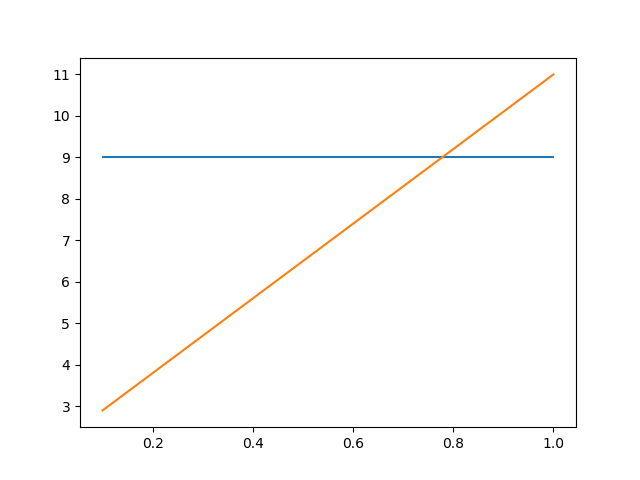
\includegraphics[scale=0.4]{ext4}
\end{frame}

\begin{frame}{Solution}
\Python{ext4}
\end{frame}

\subsection{Courbe ROC}

\begin{frame}{Receiver Operating Characteristic}

On se place dans le cas d'une classification binaire\\

\vspace{0.2cm}

On trace la courbe du nombre de vrais positifs (sensibilité) sur le nombre de faux positifs (non-spécificité) par ordre décroissant de certitude.

\end{frame}

\begin{frame}{Exemple}
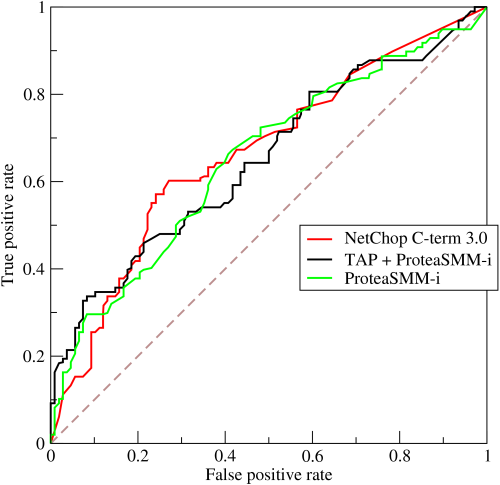
\includegraphics[scale=1.5]{ROC}
\end{frame}

\begin{frame}{Exercice}
\begin{exercice}
Avec scikit-learn, entraînez un SVM à deux valeurs sur les données du titanic en prenant uniquement l'age et le prix du billet comme variable X, et bien sûr Y pour la survie. Puis produisez la courbe ROC associées.
\end{exercice}


\end{frame}

\begin{frame}{Solution}
\Pythonsmall{ext5}
\end{frame}

\begin{frame}{Solution}
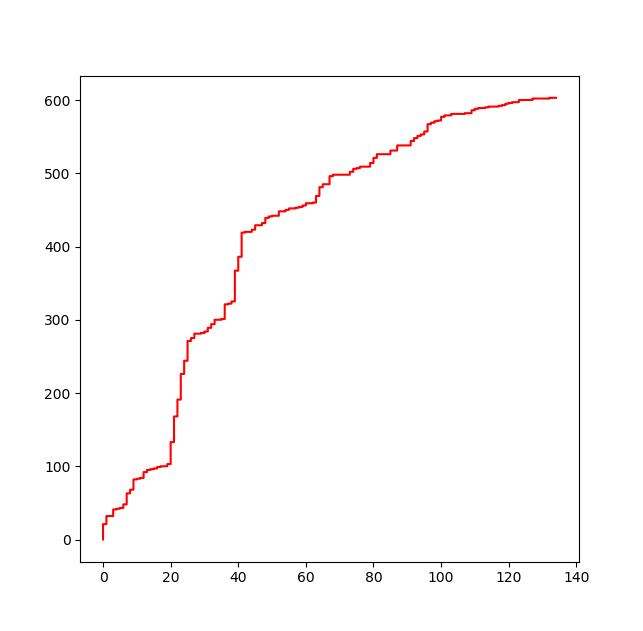
\includegraphics[scale=0.45]{ext5}
\end{frame}


\section{Risque et Consistance}

\subsection{ERM}

\begin{frame}{Erreur du modèle}

La bonne mesure serait de minimiser :

$$D(\tilde{f}) = \mathbb{E}(LF(\tilde{f}(X),Y))$$

Mais comme on ne connaît pas la loi de $(X,Y)$ c'est impossible.

\end{frame}


\begin{frame}{Erreur moyenne empirique}

On dispose d'un échantillon de test $\tau = (X_j,Y_j)_{j\leq n}$.\\

On se rabat sur l'erreur empirique :

$$\tilde{D}(\tilde{f},\tau) = \frac{1}{n}\sum_{j \leq n} LF(\tilde{f}(X_j),Y_j)$$


\end{frame}


\begin{frame}{Loi des Grands Nombres}

Si les $(X_i,Y_i)$ sont i.i.d. alors 

$$\frac{1}{n}\sum_{j \leq n} LF(\tilde{f}(X_j),Y_j) \longrightarrow \mathbb{E}(LF(\tilde{f}(X),Y))$$

\pause

\textbf{Sous cette hypothèse}, il suffit donc d'un échantillon suffisamment grand.

\end{frame}

\begin{frame}{Exercice}
\begin{exercice}
Produisez des exemples de données non i.i.d. pour lesquelles cette convergence n'existe pas.
\end{exercice}
\end{frame}


\subsection{Consistance}

\begin{frame}{Risque Optimal}
Risque théorique associé à un estimateur :
$$D(\tilde{f}) = \mathbb{E}(LF(\tilde{f}(X),Y))$$
\vspace{0.3cm}

Risque optimal :
$$ROPT = \min_{\tilde{f}}\mathbb{E}(LF(\tilde{f}(X),Y))$$

\pause

\vspace{0.3cm}

Consistance :

$$D(\tilde{f})\longrightarrow ROPT$$

\end{frame}

\begin{frame}{En résumé}
Si les $(X_i,Y_i)$ sont i.i.d. alors la moyenne empirique converge vers l'espérance du modèle

$$\frac{1}{n}\sum_{j \leq n} LF(\tilde{f}(X_j),Y_j) \longrightarrow \mathbb{E}(LF(\tilde{f}(X),Y))$$

Si le modèle est consistant alors l'espérance du modèle converge vers celle du modèle optimal

$$\mathbb{E}(LF(\tilde{f}(X),Y))\longrightarrow \min_{\tilde{g}}\mathbb{E}(LF(\tilde{g}(X),Y))$$ 
\end{frame}


\subsection{Exemple déroulé : kNN}

\begin{frame}{Algorithme}
$\sigma_x$ est une permutation sur $(X_i)$ telle que :

$$\forall i, d(X_{\sigma_x(i)},x)\leq d(X_{\sigma_x(i+1)},x)$$

$$knn(x) = argmax_{y \in Y}\mid\{x_{\sigma_X(i)},i\leq k,Y_{\sigma(i)}=y\}\mid$$
\end{frame}

\begin{frame}{Résultat}
Si $k$ est constant, knn n'est pas consistant.\\

\vspace{0.3cm}
Si $k\rightarrow \infty$ et $k/n\rightarrow 0$, knn est consistant
\end{frame}

\begin{frame}{Exercice}

\begin{exercice}
Construisez à la main un set de variables aléatoires $(X,Y)$ vérifiant une relation $Y=f(X)$, puis un jeu d'observations biaisé $(X_i)_{i\leq n},(Y_i)_{i\leq n}$ pour lequel il n'y a pas convergence de la moyenne empirique pour un 2nn. 
\end{exercice}
\begin{exercice}
Construisez à la main un set de variables aléatoires $(X,Y)$ vérifiant une relation $Y=f(X)$, puis un jeu d'observations iid $(X_i)_{i\leq n},(Y_i)_{i\leq n}$ pour lequel il y a convergence de la moyenne empitique MAIS il n'y a pas consistance de 2nn et le modèle prédit mal.
\end{exercice} 
\end{frame}

\begin{frame}{Resultat}
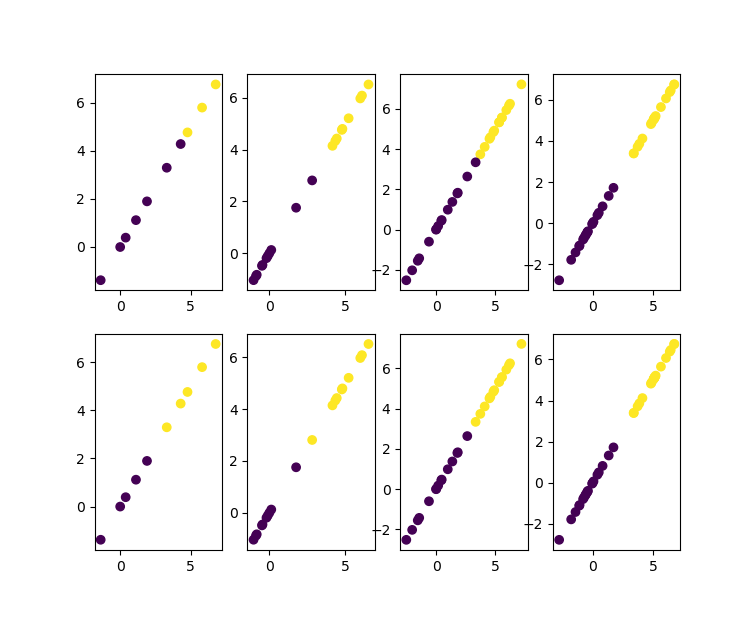
\includegraphics[scale=0.45]{ext7}
\end{frame}
\begin{frame}{Resultat}
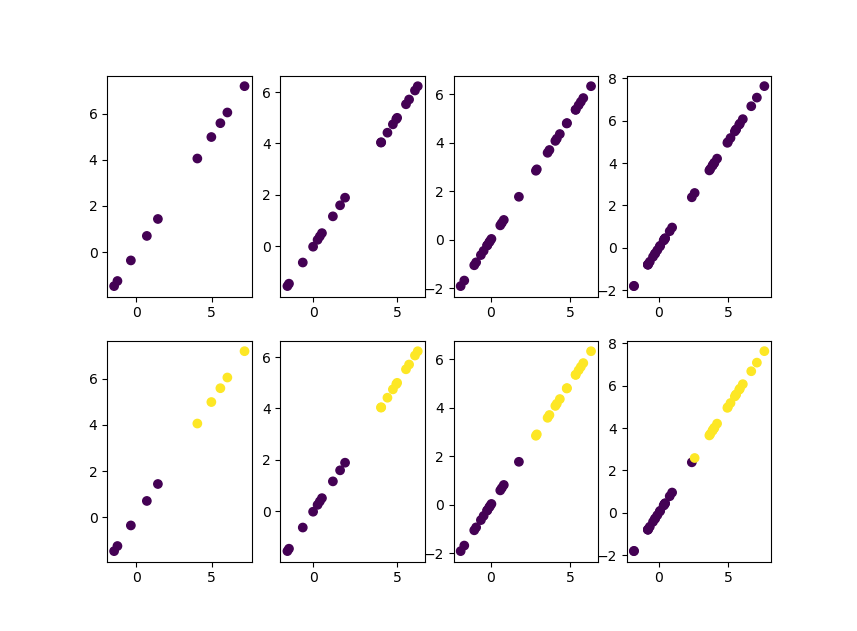
\includegraphics[scale=0.4]{ext6}
\end{frame}
\begin{frame}{Resultat}
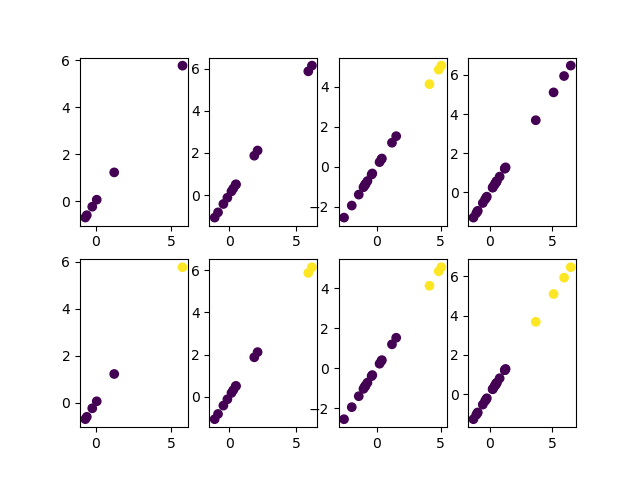
\includegraphics[scale=0.5]{ext8}
\end{frame}

\begin{frame}{Solution}
\Pythonsmall{ext6}
\end{frame}

\begin{frame}{Solution}
\Pythonsmall{ext7}
\end{frame}

\subsection{Décomposition approximation-estimation}

\begin{frame}{Minimiseur du reste empirique}

Pour :

$$\tilde{D}(\tilde{f},\tau) = \frac{1}{n}\sum_{j \leq n} LF(\tilde{f}(X_j),Y_j)$$

On peut prendre :

$$\tilde{F} = argmin_{\tilde{f}} \tilde{D}(\tilde{f},\tau)$$

\end{frame}

\begin{frame}{Décomposition du risque}
$$D(\tilde{F}) - ROPT = D(\tilde{F}) - \min_{\tilde{g}\in Z}\mathbb{E}(LF(\tilde{g}(X),Y))$$
$$+\min_{\tilde{g}\in Z}\mathbb{E}(LF(\tilde{g}(X),Y)) - ROPT $$
\end{frame}

\begin{frame}{exemples}
 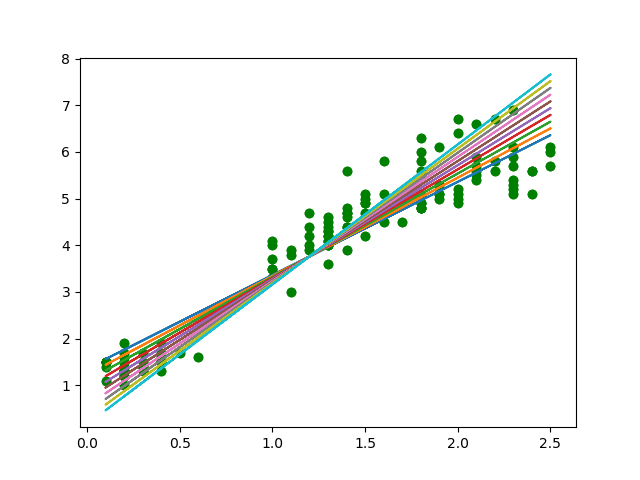
\includegraphics[scale=0.45]{ext9}
\end{frame}

\begin{frame}{exercice}
Sur l'exemple de la régression iris précédente, suggérez (et implémentez) des solutions pour réduire, soit l'approximation au détriment de l'estimation, soit l'inverse.
\end{frame}



\end{document}